Внешние расчетные нагрузки на гипотетическую конструкцию БПЛА были сформированы на основе результатов проведенных в ЦАГИ исследований \cite{BPS_TSAGI} по анализу внешних нагрузок на конструкцию БПЛА-ЦАГИ. Для предварительных расчетов прочности гипотетической конструкции БПЛА в рамках данной работы использовался один расчетный случай нагружения А, который оказался наиболее критичным для основных силовых элементов центроплана и зоны стыка крыла и фюзеляжа. 

Для силовых элементов конструкции носовой и концевой части фюзеляжа были сформированы еще два случая нагружения. 


Для основного случая нагружения основные параметры, формирующие внешнее нагружение следующие: нормальная перегрузка $n_y = 2.97$, $M = 0.4$, скоростной напор $q = 503 \text{кгс}/\text{м}^2$, высота полета $H = 6.5\text{км}$. Нагрузки на гипотетическую конструкцию БПЛА получены на основе пересчета из работы \cite{BPS}.

Эпюры аэродинамических нагрузок на крыло представлены на Рис.\ref{fig:BendingMoments},\ref{fig:RotatingMoments}.


\begin{figure}[H]
\centering
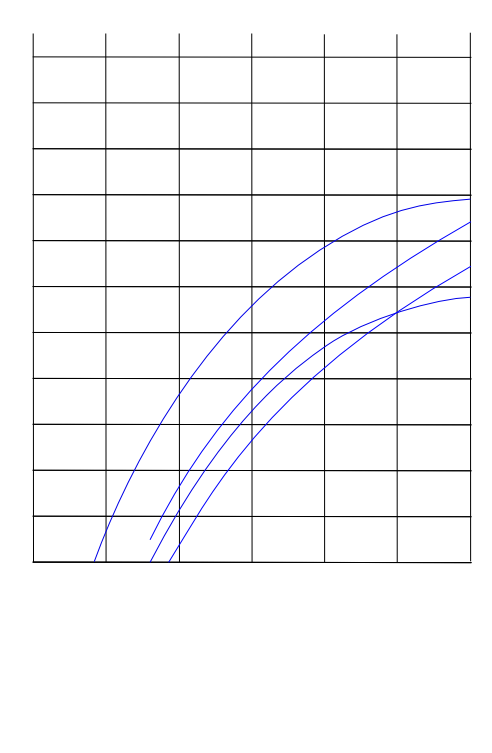
\includegraphics{HeightGraph}
\caption{Ограничения на расчетные режимы полета (случай А)}
\label{fig:ModeOfFlight}
\end{figure}


%уточнить, что где, подписать адекватно. Понять! Обозначить случай, который считаем. 

%\begin{figure}[H]
%\centering
%\def\svgwidth{0.9\textwidth}
%\input{figures/Heights.pdf_tex}
%\caption{Ограничения на режимы полета}
%\label{fig:ModeOfFlight}
%\end{figure}


\begin{figure}[H]
\centering
\def\svgwidth{0.9\textwidth}
\input{figures/BendingMoments.pdf_tex}
\caption{Эпюра изгибающих моментов}
\label{fig:BendingMoments}
\end{figure}


%\begin{figure}[H]
%\centering
%\def\svgwidth{0.9\textwidth}
%\input{figures/BendingAndRotatingMoments.pdf_tex}
%\caption{Эпюры изгибающих и крутящих моментов}
%\label{fig:BendingAndRotatingMoments}
%\end{figure}

%\begin{figure}[H]
%\centering
%\def\svgwidth{0.9\textwidth}
%\input{figures/CuttingForces.pdf_tex}
%\caption{Эпюра перерезывающих сил}
%\label{fig:CuttingForces}
%\end{figure}

%\begin{figure}[H]
%\centering
%\def\svgwidth{0.9\textwidth}
%\input{figures/DistributedLoad.pdf_tex}
%\caption{Эпюра погонной нагрузки}
%\label{fig:DistributedLoad}
%\end{figure}

\begin{figure}[H]
\centering
\def\svgwidth{0.9\textwidth}
\input{figures/RotatingMoments.pdf_tex}
\caption{Эпюра крутящих моментов}
\label{fig:RotatingMoments}
\end{figure}


Как видно из имеющихся данных (Рис.\ref{fig:BendingMoments}--\ref{fig:RotatingMoments}), влияние кручения на крыло невелико по сравнению с изгибом. В связи с этим в дальнейшем в работе при решении некоторых модельных задач будет целесообразно пренебрегать кручением крыла, рассматривая только изгибные деформации. 

